\section{Implementation}
\label{sec:imple}

\subsection{Simulation Environment}

The system is simulated in Gazebo~\cite{koenig2004gazebo}, with the hydrodynamics and the waves of the Virtual RobotX environment~\cite{bingham2019vrx}, in which the WAM-V floats on a wave field that makes it heave, roll and pitch. The x500 is flown by PX4 in software-in-the-loop, so that the NMPC drives it through the same autopilot as on the real vehicle. The tether is simulated with MoorDyn~\cite{hall2015moordyn}, as a chain of $30$ lumped masses connected by elastic segments, with the weight and the drag of the tether at the nodes, so that it hangs, goes slack and pulls on both vehicles through its own dynamics rather than through the model of the controllers. A virtual winch on the deck adjusts its length to keep the slack ratio $\varepsilon_0 = 5\,\%$, at up to $2\,\text{m/s}$, and can pull the UAV towards the deck with a constant force, to hold it during the takeoff and the landing. Wind acts on the UAV as a drag force with gusts. All the components communicate through ROS~2, and the state of both vehicles is taken from the simulator.

\subsection{Model Validation}

The models of Section~\ref{sec:model} were compared with the simulator using its nominal parameters, without fitting them to the validation data, as they are used by the controllers: over predictions of the length of each horizon, started from the state of the simulator and driven by the recorded commands. Table~\ref{tab:validation} summarises the errors at the end of the horizons. The model of the WAM-V predicts its position within $1.4\,\text{cm}$ over $2\,\text{s}$, less than $2\,\%$ of its length at the worst. The model of the x500 predicts its position within $11\,\text{cm}$ over the up to $8\,\text{m}$ it travels in $1\,\text{s}$, and the delays of the attitude response reduce the error of the attitude from about $5\,\%$ to below $1.5\,\%$ of its range. The model of the tether reduces the error of the force by $72\,\%$ and $76\,\%$ relative to a taut tether and to a hanging load, to $0.25\,\text{N}$, $1.2\,\%$ of the weight of the UAV.

\begin{table}[t]
    \centering
    \caption{Errors of the models against the simulator (RMSE, and NRMSE relative to the range of each signal).}
    \label{tab:validation}
    \footnotesize
    \begin{tabular}{@{}llrr@{}}
        \toprule
        Model & Quantity & RMSE & NRMSE \\
        \midrule
        WAM-V, $2\,\text{s}$ & position & $1.4\,\text{cm}$ & $0.37\,\%$ \\
         & heading & $0.16^\circ$ & $0.33\,\%$ \\
        x500, $1\,\text{s}$ & position & $10.8\,\text{cm}$ & $1.34\,\%$ \\
         & velocity & $0.17\,\text{m/s}$ & $2.02\,\%$ \\
         & roll, pitch & $0.63^\circ$, $0.40^\circ$ & $1.32$, $0.89\,\%$ \\
        Tether force & model & $0.25\,\text{N}$ & $10.8\,\%$ \\
         & taut tether & $0.90\,\text{N}$ & $38.9\,\%$ \\
         & hanging load & $1.03\,\text{N}$ & $44.7\,\%$ \\
        \bottomrule
    \end{tabular}
\end{table}

\subsection{Manoeuvres and Missions}

The controllers follow references, but do not decide where each vehicle should go. This is the role of the manoeuvres, which give the reference of one vehicle over the horizon of its controller at every instant. The UAV can take off, fly in formation at a point relative to the USV, in its axes or in fixed axes, orbit the USV or a point in the world, chase a target, and land, and the USV can hold its position, follow a route, pursue a target, and support the UAV from the water, following the point below it pushed away from a structure, so that it gives the UAV the reach of the tether. Since the controllers keep the vehicles within their limits, the references can remain simple, often a single point. Figure~\ref{fig:catalogue} shows the manoeuvres of the UAV as flown in the missions.

\begin{figure*}[t]
    \centering
    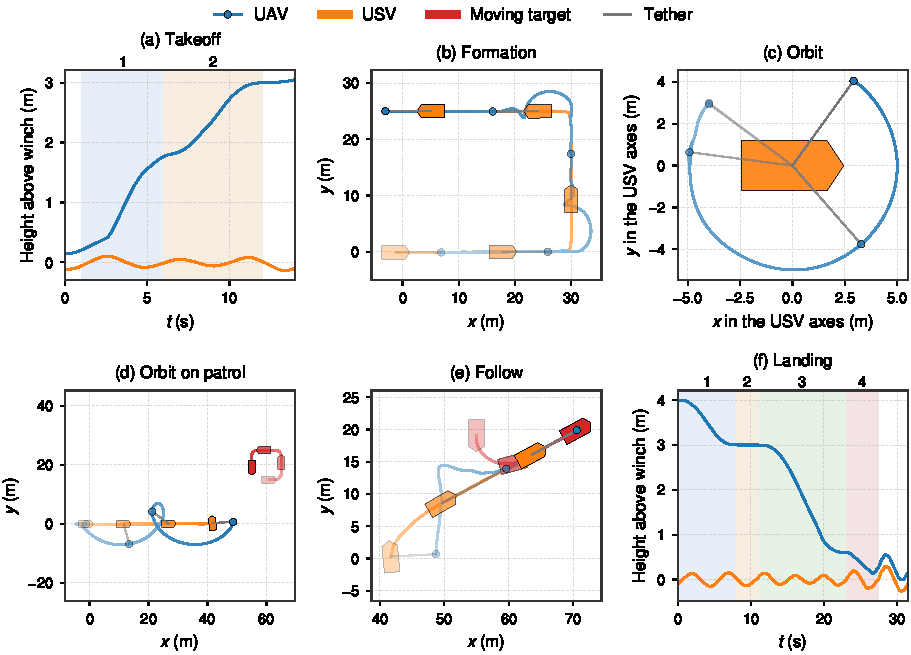
\includegraphics[width=0.85\textwidth]{Implementation/figures/04_maneuvers_and_missions/maneuver_catalogue.pdf}
    \caption{Manoeuvres of the UAV in simulation: takeoff (a) and landing (f) through the height of the UAV above the winch, with their phases, and formation (b), orbit (c, in the axes of the USV), orbit on patrol (d) and chase (e) from above, with the positions of the vehicles and the tether at several instants.}
    \label{fig:catalogue}
\end{figure*}

The takeoff and the landing are the manoeuvres in which the UAV is closest to the deck and moves with it. The takeoff starts with a vertical climb while the winch holds the UAV against the deck, so that it does not drift over its edge at low height. In the landing, the UAV first waits above the pad until it is centred and moving with it, then descends with the winch pulling it, and ends with a slow approach towards a point below the deck, so that it touches down even if the deck falls away.

A mission is a file with a sequence of manoeuvres for each vehicle, in which each manoeuvre ends with an event, such as the detection of a target, or with the end of a manoeuvre of the other vehicle. Three missions were tested: a scout, in which the UAV flies ahead of the bow while the USV follows a route, an inspection, in which the UAV circles a tower while the USV supports it, and a patrol, in which the UAV orbits the USV until it detects a target, which it then chases while the USV pursues it.

\begin{figure*}[t]
    \centering
    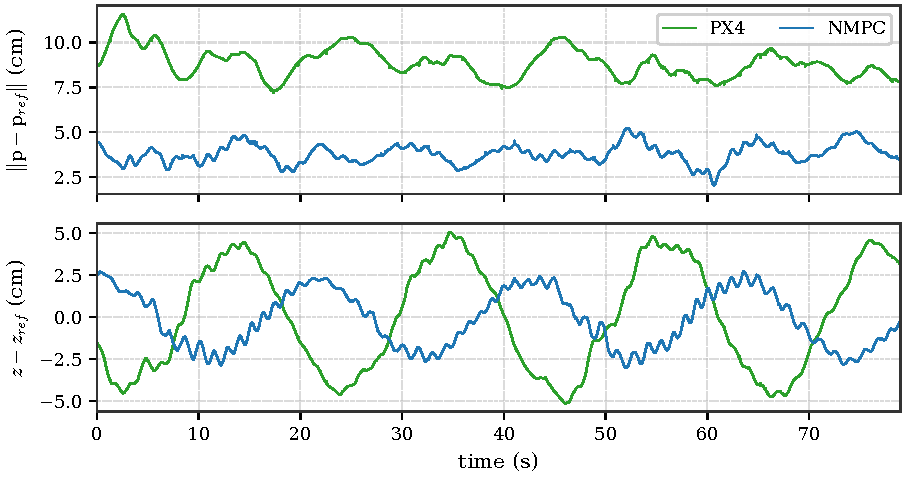
\includegraphics[width=0.8\textwidth]{Results/figures/01_tracking/nominal_error.pdf}
    \caption{Tracking error of the UAV on the tilted circle with the NMPC and with the position controller of PX4: norm of the position error and its vertical component.}
    \label{fig:nominal}
\end{figure*}
